\documentclass[letter,openrigth,12pt,spanish]{report}

%Gummi|065|=)
\title{\textbf{Intalaci\'on de ROS}}
\author{Cinematica de Robots\\
		Alcala Villagomez Mario.\\
		Becerra I\~niguez Diego Armando.\\
		Martinez Velazquez Lisbeth.\\
		Murgu\'ia Ch\'avez Nadia Sarahi.\\
		Ramos Ch\'avez Brayan Oswaldo.\\
		Ing. Mecatr\'onica 7A}
\date{13 de septiembre de 2019}

\usepackage{graphicx}

\begin{document}

\maketitle

\section{Marco Teorico}

\subsection{¿Qu\'e es ROS}

ROS (Robotic System Operating) es un middleware\footnote{Es un software que se sit\'ua entre un sistema operativo y las aplicaciones que se ejecutan en \'el. Basicamente, funciona como una capa de traducci\'on oculta que permite la comunicaci\'on y la administraci\'on de datos en aplicaciones distribuidas.} rob\'otico, es decir, una colecci\'on de frameworks\footnote{Entorno de trabajo o marco de trabajo, es un conjunto estandarizado de conceptos, pr\'acticas y criterior para enfocar un tipo de problem\'atica particular que sirve como referencia,para enfrentar y resolver nuevos problemas de \'indole similar} para el desarrollo de software de robots. ROS se desarroll\'o originariamente en 2007 bajo el nombre de switchyard por el Laboraotiro de Inteligencia Artificial de Stanford para dar soporte al proyecto del Robot con Inteligencia Artifical de Stanford (STAIR2). Desde 2008, el desarrollo continu\'o principalmente en Willow Garage, un instituto de insvestigaci\'on rob\'otico con m\'as de veinte instituciones colaborando en un modelo de desarrollo federado.\\

Apesar de no ser un sistema operativo, ROS provee los servicios est\'andar de uno de estos tales como la abstracci\'on del hardware, el control de dispositivos de bajo nivel, la implementaci\'on de funcionalidad de uso com\'un, el paso de mensajes entre procesos y el mantenimiento de paquetes. Est\'a basado en una arquitectura de grafos\footnote{Representaci\'on simb\'olica de los elementos constituidos de un sistema o conjunto, mediante esquemas gr\'aficos} donde el procesamiento toma lugar en los nodos que pueden recibir, mandar y multiplexar mensajes de sensores, actuadores, control, estados y planeaciones, entre otros. La librer\'ia est\'a orientada para un sistema UNIX (ubuntu-Linux) aunque tambi\'en se est\'a adaptando a otros sistemas operativos como Fedora, Mac OS X, Arch, Gentoo, OpenSUSE, Slackware, Debian o Microsoft Windows, cosiderando a d\'ia de hoy como 'experimentales'.\\

ROS tiene dos partes b\'asicas: la parte del sistema operativo, ros, y ros.pkg. Esta ultima consiste en una suite de paquetes aportados por la contribuci\'on de usuarios (organizadores en conjunto llamados pilas o en ingles stacks) que implementan las funcionalidades tales como localizaci\'on y mapeo simult\'aneo, planificaci\'on, percepci\'on, simulaci\'on, etc.\\

ROS es software libre bajo t\'erminos de licencia BSD. Esta licencia permite libertad para uso comercial e investigador. Las contribuciones de los paquetes en ros-pkg est\'an bajo una gran variedad de licencias diferentes.\\

Aunque est\'a en proceso de desarrolloo de aplicaciones, las \'areas que ya incluye ROS son:\\

$\diamond$ Un nodo principla de coordinaci\'on\\

$\diamond$ Publicaci\'on o subcripci\'on de datos: im\'agenes, est\'ereo, l\'aser, actuador, contacto, etc.\\

$\diamond$ Multiplexaci\'on de la informaci\'on.\\

$\diamond$ Creaci\'on y destrucci\'on de nodos.\\

$\diamond$ Los nodos est\'an perfectamente distribuidos, permitiendo procesamiento distribuido en m\'ultiples n\'ucleos multiprocesamiento, GPUs y cl\'usteres\footnote{Se usa para definir a la agrupaci\'on o conjunto de mepresas, marcas u organizaciones que suman fuerzas para aprovechar sus diferentes especializaciones con el fin de poseer ciertas vetnajes sobre la competencia, as\'i como reducir costes y mejorar su productividad.}.\\

$\diamond$ Log\'in.\\

$\diamond$ Par\'ametros de servidor.\\

$\diamond$ Testeo de sistemas.\\

En las futuras versiones se espera que las siguientes \'areas vayan apareciendo entre las palicaciones de los procesos de ROS:

$\diamond$ Percepci\'on.\\

$\diamond$ Identificaci\'on de objetos.\\

$\diamond$ Segmentaci\'on y reconocimiento.\\

$\diamond$ Reconocimiento facial.\\

$\diamond$ Reconocimiento de gestos.\\

$\diamond$ Seguimientos de objetos.\\

$\diamond$ Egomoci\'on.\\

$\diamond$ Compresi\'on de movimiento.\\

$\diamond$ Estructura de movimientos (SFM).\\

$\diamond$ Visi\'on est\'ereo: percepci\'on de profundidad mediante el uso de dos c\'amaras.\\

$\diamond$ Movimientos.\\

$\diamond$ Robots m\'oviles.\\

$\diamond$ Control.\\

$\diamond$ PLanificaci\'on.\\

$\diamond$ Agarre de objetos.\\

Entre algunos de los robots que ya utilizan ROS se pueden encontrar:

$\diamond$ \textbf{PR1}: robot personal que est\'a siendo desarrollado por Willow Garage.\\

$\diamond$ \textbf{PR2}: robot personal que est\'a siendo desarrollado por Willonw Garage.\\

$\diamond$ \textbf{Baxter}: de Rethink, Inc.\\

$\diamond$ \textbf{Robot de Shadow}: mano rob\'otica diestra motorizada desarrolalda por la empresa Shadow y la cual est\'a desarrollando mediante el consorcio de un proyecto europeo dentro del marco europeo. Entre los participantes de este proyecto se puede encontrar la empresa Shadow Robot, la Universit\'e Pierre et Marie Curie-Paris (Francia).\\ 

$\diamond$ \textbf{HERB}: desarrolado en CMU dentro del progrmama de robotica personal Intel.\\
d
\subsection{Materiales}

$\diamond$ Computadora con sistema operativo Linux (o derivados).\\

$\diamond$ Conexi\'on a Internet.\\
 
\section{Descarga e Instalaci\'on}

\subsection{Descarga de los repositorios de ROS e Instalaci\'on desde temrinal}

Antes de descargar los repositorios correspondientes desde la terminal debemos saber que tendremos que configurar los repositorios de nuestro equipo. Podemos apoyarnos en la siguiente pagina:\\

\textbf{https://help.ubuntu.com/community/Repositories/Ubuntu}\\

Una vez configurando los repositorios iremos a la pagina de ROS 'https://www.ros.org/', de aqui podemos descargar todo lo necesario para la instalci\'on del programa.\\

\begin{figure}[htp]
\centering
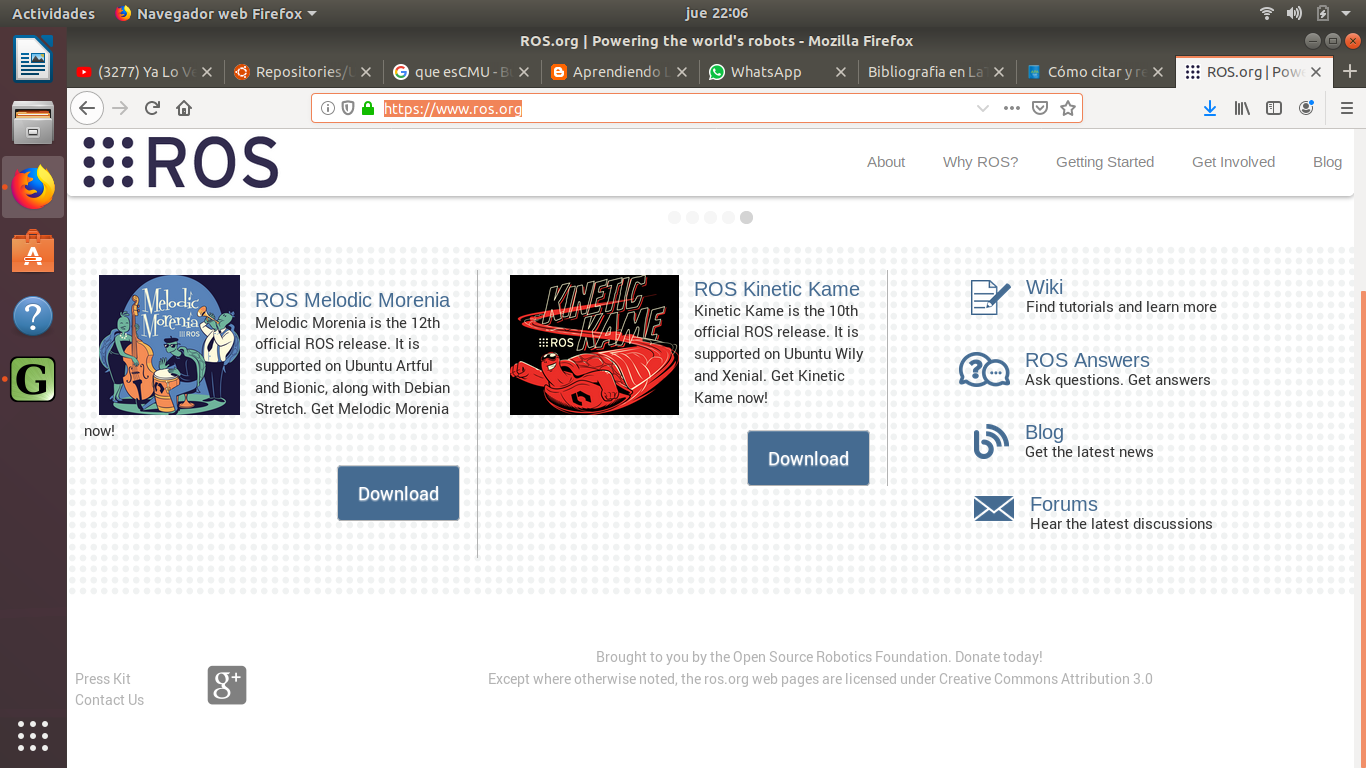
\includegraphics[width=8cm]{/home/sarha13/Escritorio/ros.png}
\caption{Pagina de ROS}
\label{Figura 1.}
\end{figure}

Despues de esto seleccionaremos la verci\'on que queramos instalar:\\

\begin{figure}[htp]
\centering
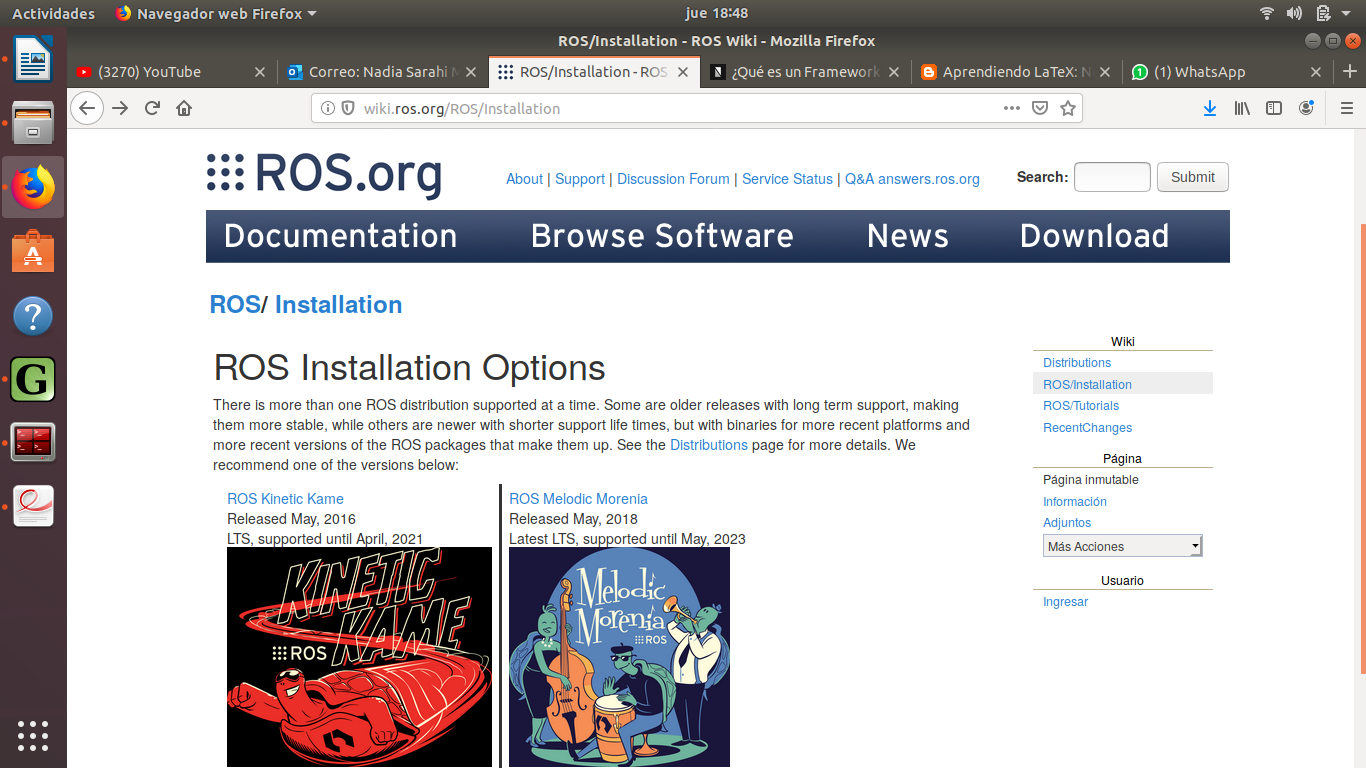
\includegraphics[width=8cm]{/home/sarha13/Escritorio/version.png}
\caption{Seleccion de version}
\label{FIgura 2.}
\end{figure}

Ya que seleccionamos la versi\'on, seleccionaremos el tipo de sistema operativo donde lo instalaremos, en este caso Ubuntu:\\

\begin{figure}[htp]
\centering
\includegraphics[width=8cm]{/home/sarha13/Escritorio/sistema.png}
\caption{Seleccion de sistema operativo}
\label{Figura 3.}
\end{figure}

Esto nos llevara la pagina donde nos marcara los pasos a seguir para la intalaci\'on atravez de la teminal de Ubuntu.\\

\begin{figure}[htp]
\centering
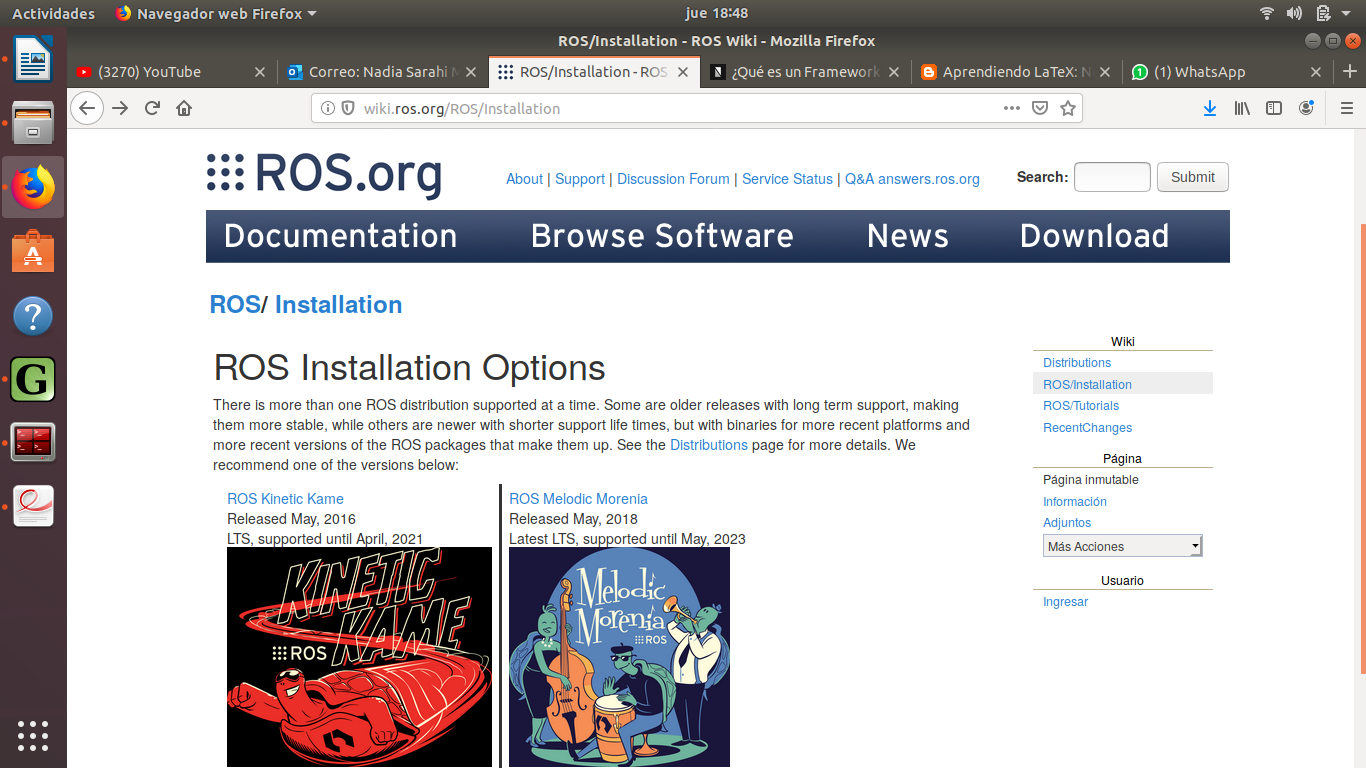
\includegraphics[width=8cm]{/home/sarha13/Escritorio/instalacion.png}
\caption{Manuel de instalci\'on }
\label{Figura 4.}
\end{figure}

Ya que tenemos el manual de inestalaci\'on para ROS abriremos la terminal de Ubuntu con la combinaicon de teclas \textbf{Ctrl+T}.\\

primero descargaremos el respositorio de ROS con el siguiente comando (todos los comandos varian despendiendo la versi\'on y son arrojados por la pagina):\\

\begin{center}
\textbf{sudo sh -c 'echo "deb http://packages.ros.org/ros/ubuntu $\$$(lsb\underline{ }release -sc) main" > /etc/apt/sources.list.d/ros-latest.list'}\\
\end{center}

\begin{figure}[htp]
\centering
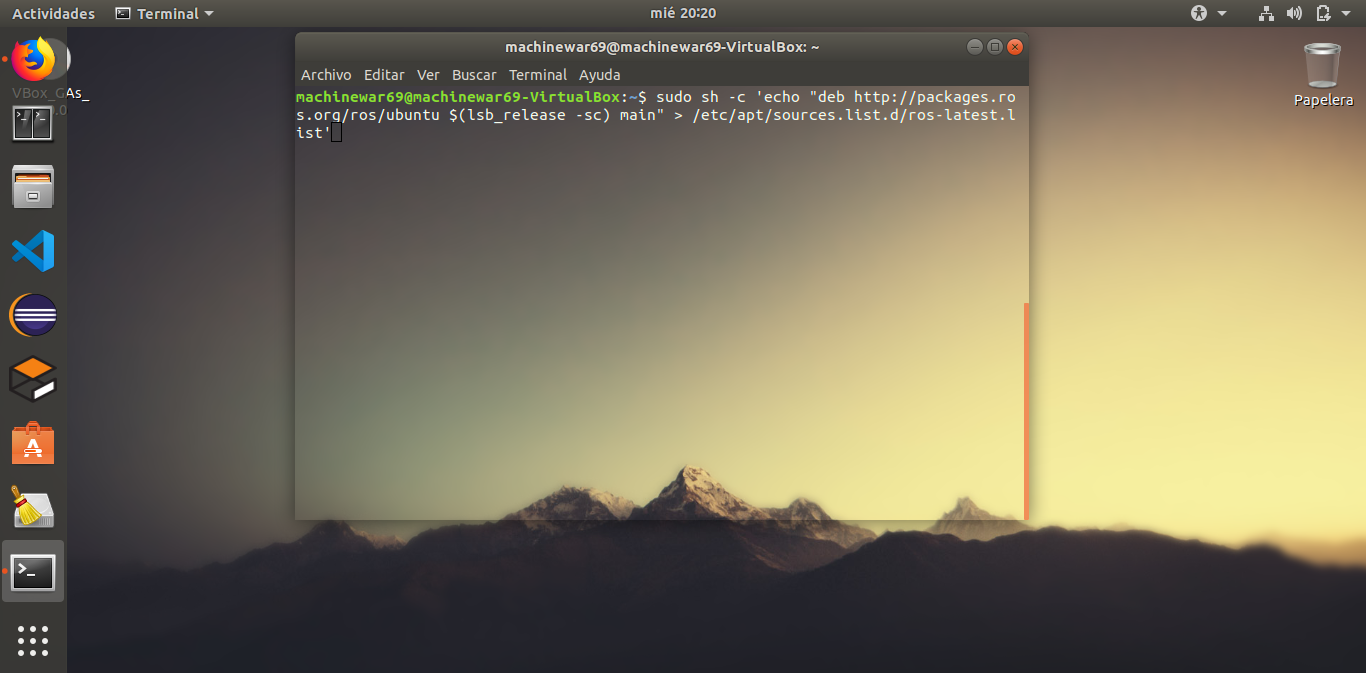
\includegraphics[width=8 cm]{/home/sarha13/Escritorio/terminal1.png}
\caption{Descarga de repositorios}
\label{Figura 5.}
\end{figure}

Una vez que se haya descargado completamente los respositorios nos conectaremos a un servidor para poder realizar la instalci\'on. Escribiendo el siguiente comando en la consola:\\

\textbf{sudo apt-key adv --keyserver 'hkp://keyserver.ubuntu.com:80' --recv-key C1CF6E31E6BADE8868B172B4F42ED6FBAB17C654}

\begin{figure}[htp]
\centering
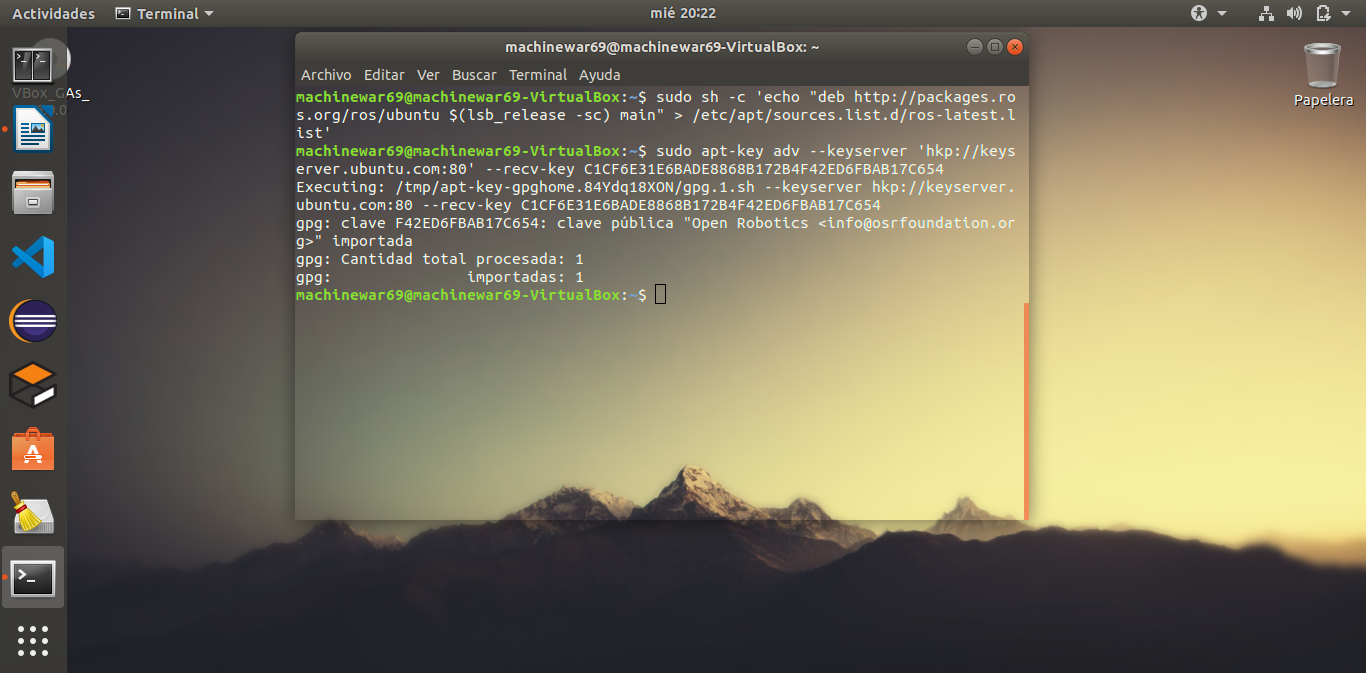
\includegraphics[width=8cm]{/home/sarha13/Escritorio/terminal2.png}
\caption{Conexi\'on al servidor}
\label{Figura 6.}
\end{figure}

Puedes utilizar le siguiente comando:\\

\textbf{curl -sSL 'http://keyserver.ubuntu.com/pks/lookup?op=get$\&$search=0xC1CF6E31E6BADE8868B172B4F42ED6FBAB17C654' | sudo apt-key add -}

Una vez conectados al servidor instalaremos ROS mediante el siguiente comando:\\

\begin{center}
\textbf{sudo apt-get update}\\
\end{center}

\begin{figure}[htp]
\centering
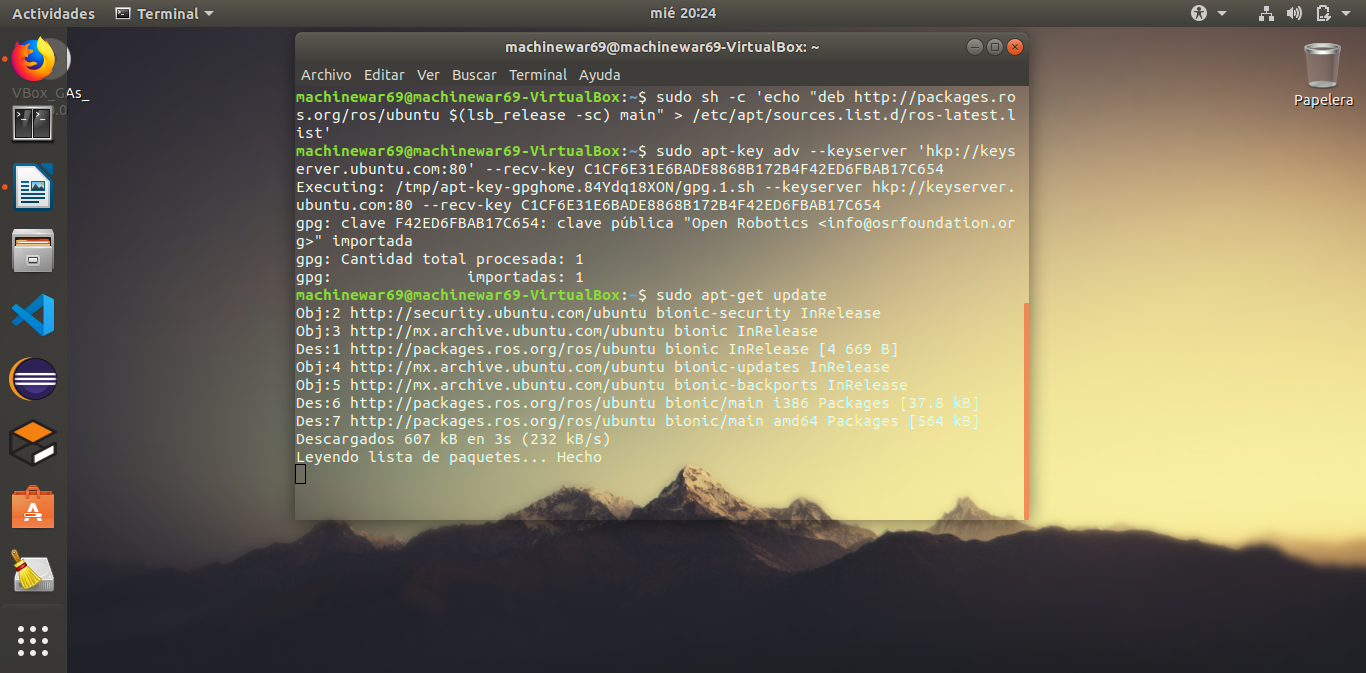
\includegraphics[width=8cm]{/home/sarha13/Escritorio/terminal3.png}
\caption{Instalacion de paqueterias de ROS}
\label{Figura 6.}
\end{figure}

Esto nos instalara ROS con todas las paqueterias que contiene, en caso de que solo se requiera de algunas librerias en la pagina puedes encontrar varias opciones de descarga. Para esto usaremos el siguietne comando nos dara la descarga de todas las paqueterias de ROS:\\

\begin{center}
\textbf{sudo apt-get install ros-kinetic-desktop-full}\\
\end{center}

\begin{figure}[htp]
\centering
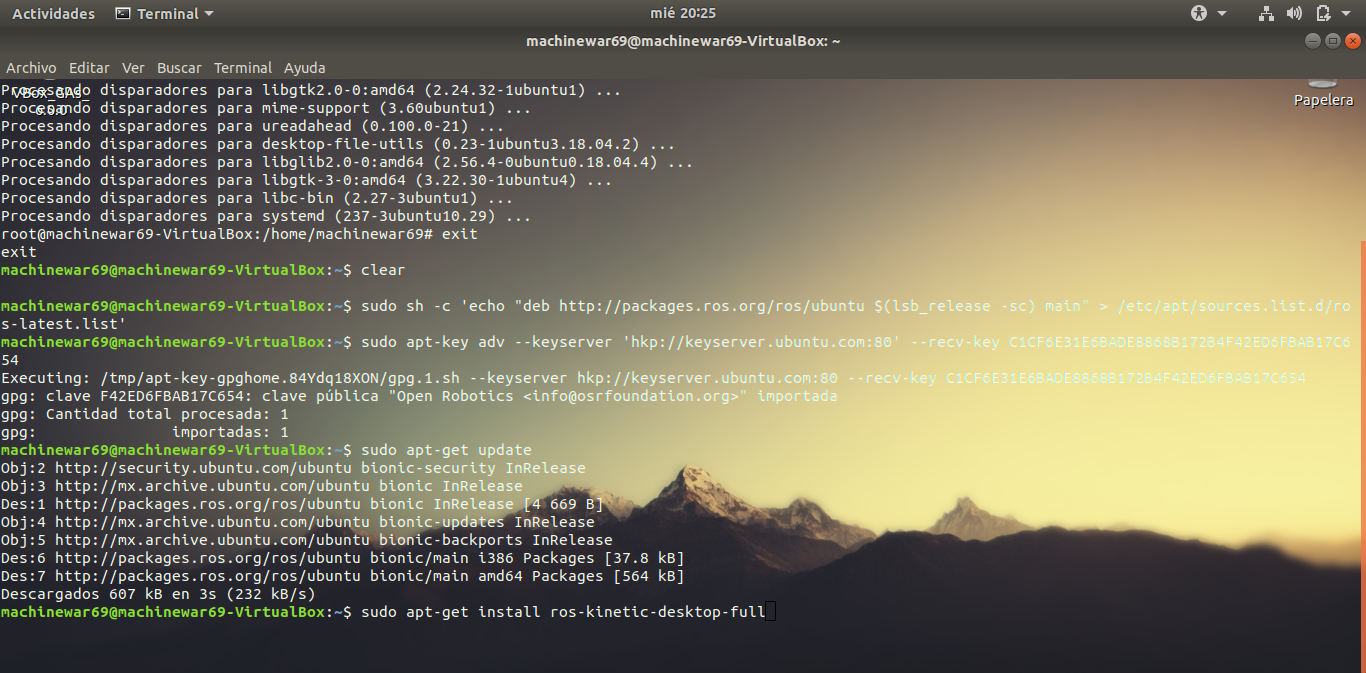
\includegraphics[width=8cm]{/home/sarha13/Escritorio/terminal4.png}
\caption{Instalacion de paqueterias}
\label{Figura 8.}
\end{figure}

Ya que se haya descargado todas la paqueterias que deseamos ingresaremos en la terminal el siguiente comando:\\

\begin{center}
\textbf{sudo rosdep init}\\
\end{center}

Esto para la inicializaci\'on de ROS, seguido del comando:\\

\begin{center}
\textbf{rosdep update}\\
\end{center}

\begin{figure}[htp]
\centering
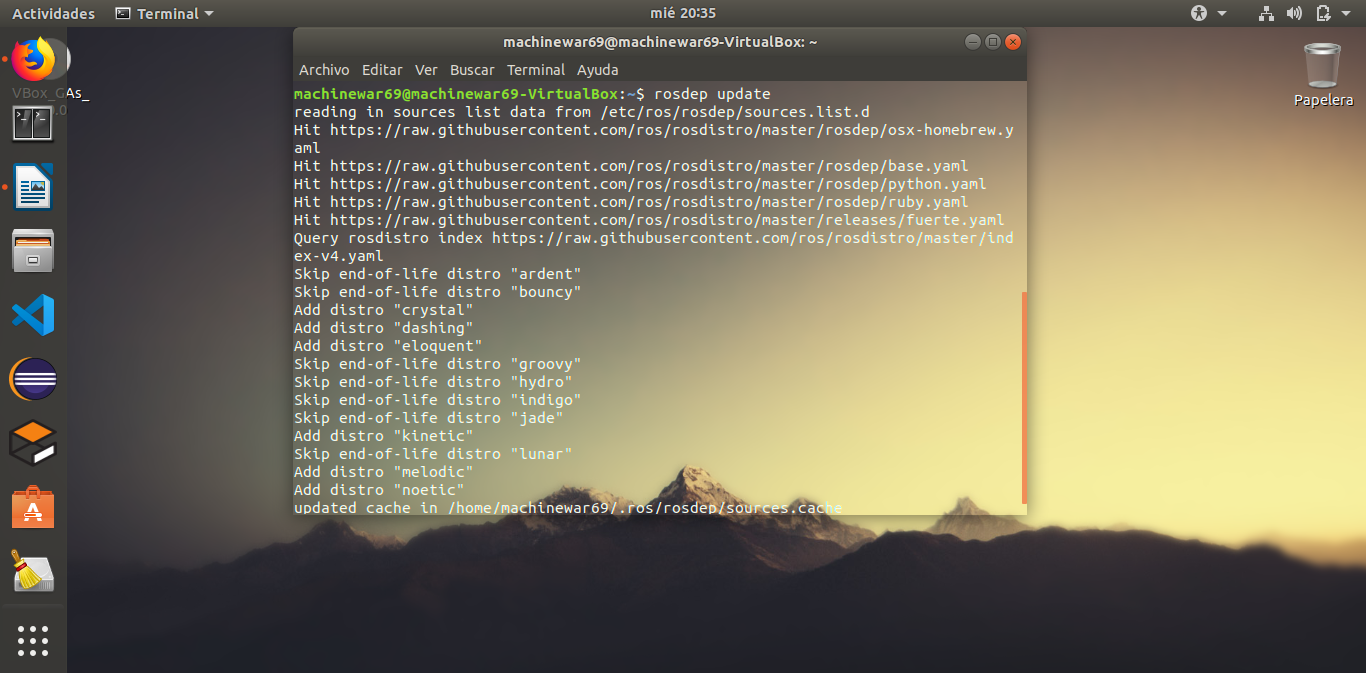
\includegraphics[width=8cm]{/home/sarha13/Escritorio/terminal5.png}
\caption{Iniciaici\'on de ROS}
\label{Figura 9.}
\end{figure}

Para terminar de iniciar ingrasaremos el archivo .bash para la finalizaci\'on de este proceso con el siguiente comendo:\\

\begin{center}
\textbf{echo "source /opt/ros/kinetic/setup.bash" >> ~/.bashrc
source ~/.bashrc}\\
\end{center}

seguido de los suguientes comandos:\\

\begin{center}
\textbf{source /opt/ros/kinetic/setup.bash}\\
\end{center}

\begin{center}
\textbf{echo "source /opt/ros/kinetic/setup.zsh" >> ~/.zshrc
source ~/.zshrc}\\
\end{center}

Una vez iniciado ROS descargaremos las dependecias correspondientes ingresando el siguiente comando:\\

\textbf{sudo apt install python-rosinstall python-rosinstall-generator python-wstool build-essential}\\

\begin{figure}[htp]
\centering
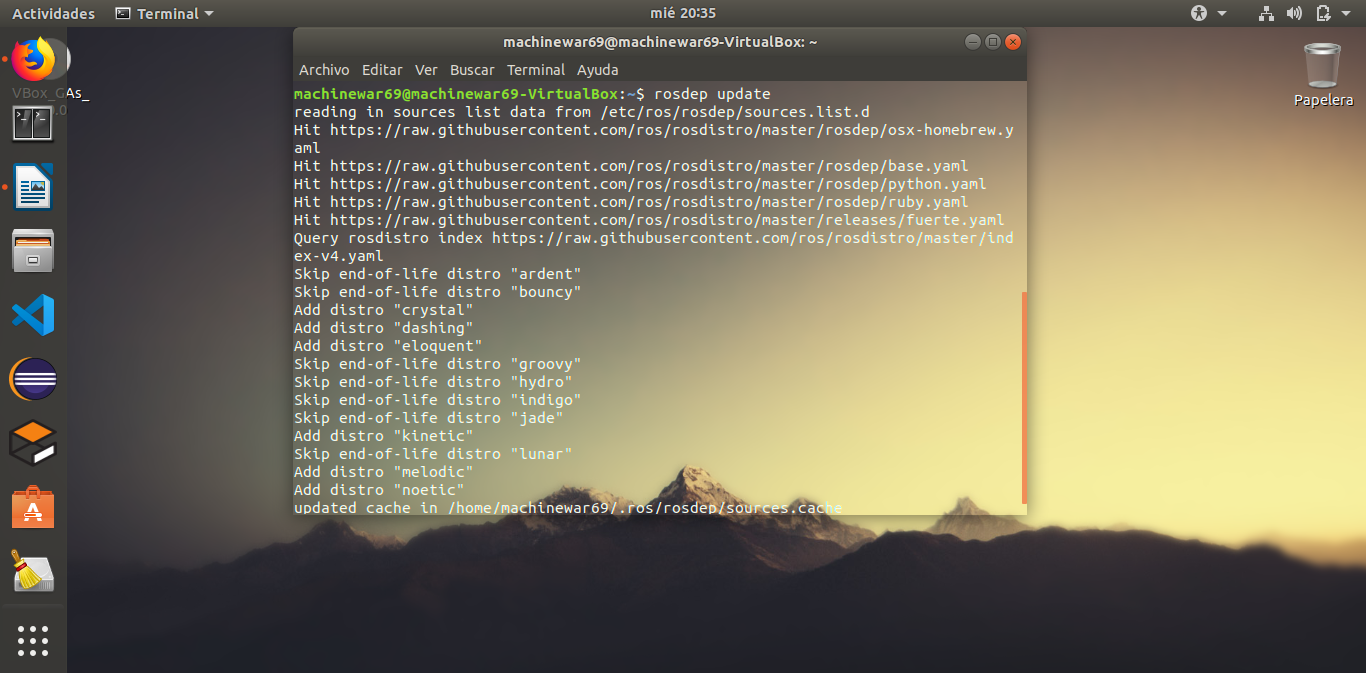
\includegraphics[width=8cm]{/home/sarha13/Escritorio/terminal5.png}
\caption{Instalaci\'on de dependencias}
\label{Figura 10.}
\end{figure}

Y con esto tenemos hemos terminado la instalaci\'on de ROS, en nuestros equipo de computo, ahora si queremos saber si se instalo bien ingresaremos el siquiente comando en la consola:\\

\begin{center}
\textbf{roscore}
\end{center}

\begin{figure}[htp]
\centering
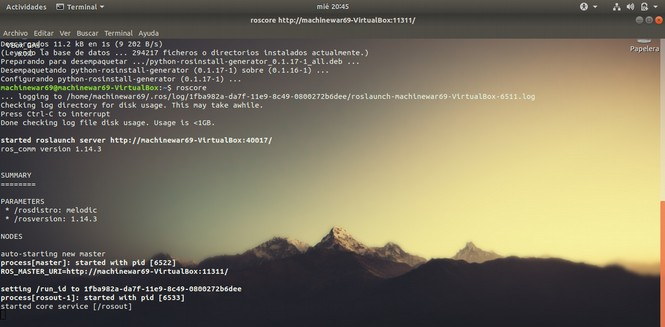
\includegraphics[width=8cm]{/home/sarha13/Escritorio/temrinal7.jpg}
\caption{Verificaci\'on de inicio}
\label{Figura 11.}
\end{figure}

Una ves comprovado que corra bien ROS hemos terminado y esta listo para utilizarce.\\

\section{Concluciones}

\textbf{Alcala Villagom\'ez Mario}:\\
El dibujo asistido por computadora ocupa un papel importante en el dibujo, conocido como CAD. El CAD es el proceso en el cual se utilizan ordenadores o computadoras para mejorar la fabricación, desarrollo y diseño de los productos, aumentando el precio, y mayor precisión en los productos. Este consta de una tabla graficadora y un software especializado en dibujo utilizando dimensiones virtuales. 

Esto hace que podamos obervar las piezas con una aproximacion mas acertada,el diseño y simulacion es vital para un buen ensamble por lo cual el uso de estas herrmientas es fundamental.\\

\textbf{Becerra Iñiguez Diego Armando}:\\
La importancia que tiene los robots actualmente ha llegado a fines insospechables. Desde las industrias hasta las oficinas podemos encontrar actividad de estos seres artificiales; sin embargo, siempre ha existido una variable con la que los ingenieros han batallado buscando mejorar. Cómo hacer que estos seres piensen y act\'uen m\'as como humanos y no como simples maquinas. La respuesta, mediante la programación, con un sistema operativo llamado ROS.La programaci\'on es relevante porque hace que los robots ejecuten tareas complejas sin m\'as contratiempo. El problema con esto radica en la complejidad de la tarea misma, es decir mientras m\'as dif\'icil y/o laboriosa fuese la actividad, la codificaci\'on es un dolor de cabeza para el desarrollador. Eso sin contar con los m\'ultiples problemas de compatibilidad de hardware que siempre se llegan a encontrar cuando queremos implementar características adicionales a nuestro robot.\\

\textbf{Martinez Velazquez Lisbeth}:\\
Uno de mis objetivos principales era lograr completar el procedimiento de la instalación del software de ros, al parecer se logr\'o completar dicho objetivo.

Los conocimientos previos sobre esta actividad fueron recordar cómo se debe instalar el software en la máquina virtual de Ubuntu además de cómo se debe interpretar y manejar para la configuración y la utilización de la Ras Berry en Ros.\\

\textbf{Murgu\'ia Ch\'avez Nadia Sarahi}:\\
Para la instalaci\'on de ROS se tiene que considerar varias cosas de las cuales son la versi\'on pues en cursos anteriores hicimos uso de ROS pero se tuvieron varias complicaciones durante su uso pues la versi\'on que se instalo anteriormente daba muchos conflictos al momento de realizar las actividades, al vovler ha realizar la instalaci\'on con otra versi\'on observamos que funciona mejor.\\

\textbf{Ramos Ch\'avez Brayan Oswaldo}:\\
En la instalación de ros se obtuvo fácilmente mediante los códigos que se obtuvieron en la página oficial de ros incorporación que se introduciremos fácil mente y que se o tuvieron resultados que la instalación de ros fue un éxito que pudimos tener la comunicación de ros en linux si problemas.\\

\newpage

\begin{thebibliography}{X}

\bibitem{ROS} \textsc{ROS.org} (2010-2018) \textsc{ROS-Install}.: Recuperado de https://www.ros.org/

\bibitem{Ubuntu} \textsc{Repositories/Ubuntu} (2015-2017) \textsc{WikiGuide}.: Recuperado de https://help.ubuntu.com/community/Repositories/Ubuntu

\bibitem{ROS} \textsc{Hipopoto S.L.} (2018-2019) \textsc{¿Qu\'e es ROS?}.: Recuperado de https://openwebinars.net/blog/que-es-ros/

\end{thebibliography}


\end{document}